\documentclass[phd,tocprelim]{cornell}
%
% tocprelim option must be included to put the roman numeral pages in the
% table of contents
%
% The cornellheadings option will make headings completely consistent with
% guidelines.
%
% This sample document was originally provided by Blake Jacquot, and
% fixed up by Andrew Myers.
%
%Some possible packages to include
\usepackage{graphicx}
%\usepackage{graphics}
%\usepackage{moreverb}
%\usepackage{subfigure}
%\usepackage{epsfig}
%\usepackage{subfigure}
%\usepackage{hangcaption}
%\usepackage{txfonts}
%\usepackage{palatino}

\usepackage{amsmath}
\usepackage{amssymb}

\DeclareMathOperator*{\argmin}{argmin}
\DeclareMathOperator*{\argmax}{argmax}

%if you're having problems with overfull boxes, you may need to increase
%the tolerance to 9999
\tolerance=9999

\bibliographystyle{plain}
%\bibliographystyle{IEEEbib}

\renewcommand{\caption}[1]{\singlespacing\hangcaption{#1}\normalspacing}
\renewcommand{\topfraction}{0.85}
\renewcommand{\textfraction}{0.1}
\renewcommand{\floatpagefraction}{0.75}

\title {Your Title Goes Here}
\author {Scott Clark}
\conferraldate {August}{2012}
\degreefield {Ph.D.}
\copyrightholder{Scott Clark}
\copyrightyear{2012}

\begin{document}

\maketitle
\makecopyright

\begin{abstract}
Your abstract goes here. Make sure it sits inside the brackets. If not,
your biosketch page may not be roman numeral iii, as required by the
graduate school.
\end{abstract}

\begin{biosketch}
Scott Clark grew up in Tigard, Oregon and graduated from Central Catholic High School in Portland, Oregon in 2004. He recieved Bachelor of Science degrees in Mathematics, Computational Physics and Physics (Magna Cum Laude) from Oregon State University in 2008.

In 2008 Scott was awarded a Department of Energy Compuational Science Graduate Fellowship (CSGF) supporting his doctoral work at Cornell University Center for Applied Mathematics (CAM). He plans to move to San Francisco after graduation and has accepted a position at Yelp Inc.
\end{biosketch}

\begin{dedication}
This document is dedicated to my family.

Your constant, unconditional love and support at every stage of my education made this possible.
\end{dedication}

\begin{acknowledgements}
I have had the priveledge of working with many amazing educators and researchers throughout my academic career. They have all helped sculpt me into the student and person I am today. At Central Catholic High School Steve Workman, Paul Wallulis and Phil Collins taught me the value of hard work and opened my eyes to the world of math and science. My REU advisors, Prof. Daniel Cox of University of California Davis and Prof. Steven Tomsovic of Washington State University. My undergraduate advisors at Oregon State, Malgo P and Rubin Landau. My practicum supervisors: Dr. Nick Hengartner and Dr. Joel Berendzen of Los Alamos National Labratory; and Dr. Zhong Wang and Rob Egan of the Joint Genome Institute of Lawerence Berkeley National Labratory. My committee at Cornell: Prof. Steve Strogatz and Prof. Bart Selman. And, of course, my advisor Prof. Peter Frazier whose unwavering patience, support and encouragement made this possible.

And my family and friends...

My research was supported by a Department of Energy Computational Science Graduate Fellowship, which is supported by the Office of Science of the U.S. Department of Energy under Contract No. DE-FG02-97ER25308. I was also supported by a Startup and Production Allocation Award from the National Energy Research Scientific Computing Center (NERSC), which is supportedby the Office of Science of the U.S. Department of Energy under Contract No. DE-AC02-05CH11231.
\end{acknowledgements}

\contentspage
\tablelistpage
\figurelistpage

\normalspacing \setcounter{page}{1} \pagenumbering{arabic}
\pagestyle{cornell} \addtolength{\parskip}{0.5\baselineskip}

\part{ALE: Assembly Likelihood Evaluation} % (fold)
\label{prt:ALE: Assembly Likelihood Evaluation}

\chapter{ALE Introduction} % (fold)
\label{cha:ALE Introduction}

Recent advances in metagenomics have enabled the study of the microbes directly from complex communities implicated in environment and health {Tringe, 2005}.  DNA extracted from microbial communities can be investigated either by 16S rDNA sequencing to explore their phylogenetic diversity {Costello 2009;}, or by whole metagenome shotgun sequencing to understand their full genetic constituents {Venter 2004; Tringe 2005;Qin 2010;Yooseph 2010; Hess 2011}. With the unprecedented amount of data obtained from next generation highthroughput sequencing (NGS), individual genomes can be directly assembled from a mixture of thousands of genomes, without the need to isolate single genomes through laboratory cultivation or single cell sorting {Hess, 2011}. The ability to assemble a metagenome to resolve the genomes of individual species, or at least the abundant ones from a complex community, is crucial to understanding their community structure and dynamics and to exploring inter-species interactions, thereby providing deeper insights into the function of the community. 

Assembly of individual genomes from metagenomics datasets generated by NGS poses significant informatics challenges. Many of these challenges, including short read length, noisy data and large data volume, are also faced in the assembly of single large genomes from short reads (reviewed in {Lin 2011; Li 2010}). Beyond those faced in assembling single genomes, there are also several challenges unique to metagenome assembly. First, unlike in single genome assembly where the sequence depth for the target genome is expected to be uniform, the sequencing depth of genomes in a metagenome usually vary greatly. Second, most genome assemblers have difficulties in resolving repetitive regions within a single genome, and this problem is exacerbated in metagenome assembly because conserved genomic regions and lateral gene transfer have greatly increased the portion of the “repetitive” genomic regions. Finally, although there are quite a few single genome assemblers such as Velvet {Zerbino and Birney 2008}, ABySS {Simpson et al 2009}, soapDenovo {Li 2010} and All-Path-LG {Gnerre et al 2010} that are capable of assembling large genomes, there is no metagenome specific assembler yet. Instead, assemblers designed for single genomes are being applied to metagenome data without significant modifications {Qin 2010; Hess 2011}. The impact of using an assembler developed to assemble single genome has not yet been systematically evaluated for metagenome assembly, especially in how well it addresses challenges like variable sequencing depth and closely related species that are unique to metagenomes. Quantitative measurement of the quality of a metagenome assembly, as well as the ability to compare the results of different assemblers from the same data set, are so far impossible. Many current studies either use only the overall size of assembly (N50), which ignores accuracy, or maps the resulting assembly onto some known reference genomes obtained independently to estimate the accuracy {Hess 2011}, but such references are not available in most cases. In this work we focus on the accuracy of the proposed genome using only the proposed assembly and the reads used to create it. This allows us to pinpoint localized errors instead getting bogged down trying to quantify the completeness of an entire metagenome.

Quality measurements of a single genome assembly have been derived by using a basic statistical framework integrating several metrics {Lin 2011; }. These metrics in general include the completeness (the total assembled bases), the contiguity (N50), and the accuracy (how well the assembly is supported by the reads and mate pairs) {Li 2010}. The first two often improve as the sequencing depth increases, and the accuracy at the base level is also correlated with sequence depth. However, accuracy at the contig/scaffold level is often independent of sequence depth, as chimeras can form by mis-joins and repeats regions can be misplaced and miscounted, which requires additional assessments. Such assessments can be derived from the original reads that formed the assembly, for example, by mapping the reads back to the proposed assembly {Zhong, Rob: REF? Maybe bowtie?}. Good assemblies require mate pairs to map to the same loci, insert length to be normally distributed around the mean, and most reads to map onto the assembly {Zhong, Rob: REF? Or common knowledge?}. Additionally they require that when reads are mapped onto the assembly their coverage, or depth, must be consistent with the Poisson distribution, which follows from a random shearing process {Lander 1988}. Unfortunately these requirements may not be directly applied to evaluate metagenome assembly quality. For example, single genome assemblies require all read pairs to be oriented consistently by the assumption a single genome, a constraint not followed when dealing with metagenome assemblies because read pairs can map to similar regions on different genomes.

In this work we aim to provide a comprehensive integrated framework for evaluating the quality of single genome and metagenome assemblies.  In related work, {Phillipy 2008} also proposed a method for evaluating the quality of a whole single genome, but the method proposed is a pipeline of conceptually separate techniques for evaluating the different aspects of genome quality.  {Choi 2008} also combined evidence from several conceptually separate measures of genome quality to identify mis-assemblies.  In the previous literature, those works that use a single statistical framework tend to focus on only a single aspect of genome quality: {Zimin 2008} introduced a metric (CE statistic) for finding gaps in an assembly by comparing to the genome of a related organism; {Meader 2010} developed a statistical method for estimating the rate of erroneous insertions and deletions present in an assembly by comparison to an assembly of a closely related species; {Olson 2009} uses mate pair information and a reference genome from a similar organism to identify assembly errors and structural variation;  {Kelly 2010} introduced a method that detects false segmental duplication using mate pair and coverage information.  All of these previous approaches contrast with the current work, which is an integrated method for validating several aspects of genome and metagenome assembly quality simultaneously based on a single statistical model.  Like the current work, {Laserson 2011} also used a single statistical model to assign a likelihood score to assemblies, focusing specifically on the metagenomic case, but the statistical model used ignores the role of mate pairs in assessing assembly quality, which are becoming more prevalent with NGS technologies such as Illumina and PacBio “strobe” reads..

In this work, we measure the overall quality of an assembly in a mathematically rigorous way, using a probabilistic model for the way that reads are generated from a genome.  Using Bayesian statistics, we give explicit expressions for the probability that an assembly is correct, and computational methods based on these expressions.  These mathematical methods avoid the pitfalls of summary statistics like N50 score, which only capture one dimension of assembly quality.
The methods provided may be used in a number of ways.  First, they are useful as a tool for comparing different assemblies of the same genome or metagenome, and can be used to show how much more likely one assembly is than another of being correct.  Two assemblies with roughly equal likelihood of correctness can be considered as having roughly equal quality, while if one assembly has a likelihood that is much lower, then we may safely discard it as inferior.  Second, when considering a single assembly in isolation, these methods can also be used to give an absolute score that indicates the quality of this assembly, and how this quality compares to the quality of other assemblies.  Third, these methods can be used to examine a single assembly and identify errors and their location, which is particularly useful when finishing the assembly.

% chapter ALE Introduction (end)

\chapter{ALE Methods} % (fold)
\label{cha:ALE Methods}

\section{The ALE Score and the likelihood of an assembly} % (fold)
\label{sec:The ALE Score and the likelihood of an assembly}

The ALE framework is founded upon a statistical model that describes how reads are generated from an assembly.  Given a proposed assembly (a set of scaffolds or contigs), S, and a set of reads R, this probabilistic model gives the likelihood of observing this set of reads if the proposed assembly were correct.  We write this likelihood, $P(R|S)$, and its calculation includes information about read quality, agreement between the mapped reads and the proposed assembly, mate pair orientation, insert length (for paired end reads), and sequencing depth.  This statistical model also provides a Bayesian prior probability distribution $P(S)$ describing how likely an assembly $S$ would be, if we were unable to observe any read information.   This prior probability is computed using the k-mer distribution of the assembly.

The ALE score is computed from these two values, and it is proportional to the probability that the assembly S is correct.  We write this probability as $P(S|R)$.  Bayes’ rule tells us that this probability is
\begin{equation}
    P\left(S|R\right) = \frac{P\left(S|R\right)P(S)}{Z}
\end{equation}
where Z is a proportionality constant that ensures that P(S|R) is a probability distribution.  We see P(S|R) as a statistical measure of the overall quality of an assembly S.  As is typical in large-scale applications of Bayesian statistics, it is computationally intractable to compute the constant Z exactly.  The ALE score is computed by replacing the constant Z with an approximation described in the Methods section.

Although the ALE score can be reported as a standalone value, and understood as an approximation to P(R|S), it is most useful for comparing two different assemblies of the same genome, using the same set of reads to evaluate them.  As shown in the Methods section, the assembly with the higher ALE score is then also the one with the larger probability of being correct.  Moreover, we show that the difference between two assemblies’ ALE scores describes their relative probabilities of correctness.  If one assembly’s ALE score is larger than the other’s, with a difference of x between their ALE scores, then the assembly with the larger ALE score is more likely to be correct by a multiplicative factor of ex.  Below, we refer to the ALE score more precisely as the total ALE score, to differentiate it from the sub-scores (described below) used to construct it.

Figure 1 shows the pipeline used to compute the total ALE score. Given a set of reads and a proposed assembly, ALE first takes as input the alignments of the reads onto the assembly in the form of a SAM or BAM file (Li and Durbin 2009), which can be produced by a third-party alignment algorithm such as bowtie (Langmead et al. 2009) or bwa (Li et al. 2009). ALE then determines the probabilistic placement of each read and a corresponding placement sub-score for each mapped base, which describes how well the read agrees with the assembly.  In the case of paired end reads, ALE also calculates an insert sub-score for all mapped bases of the assembly from the read pair, which describes how well the distance between the mapped reads matches the distribution of lengths that we would expect from the library.  ALE also calculates a depth sub-score, which describes the quality of the sequencing depth accounting for the GC bias prevalent in some NGS techniques.  The placement, insert and depth scores together determine P(R|S).  Independently, with only the assembly and not the reads, ALE calculates the k-mer sub-score and P(S). Each sub-score is calculated for each scaffold or contig within an assembly independently, allowing for variations commonly found in metagenomes. The four sub-scores are then combined to form the total ALE score. The constituent calculations in this pipeline are described in the Methods section.

In addition, these four sub-scores are reported by ALE as a function of position within the assembly, and can be visualized with the included plotting package or imported in table form to another package such as the Integrative Genomics Viewer (IGV) (Nicol et al. 2009), or the UCSC genome browser (Kent et al. 2002).  When used in this way, these sub-scores can be used to locate specific errors in an assembly.

% section The ALE Score and the likelihood of an assembly (end)

\section{Probabilistic ingredients of the total ALE score} % (fold)
\label{sec:Probabilistic ingredients of the total ALE score}

We can combine the two probabilities, $P(R|S)$ and $P(S)$, to provide an expression for the probability of the assembly given the reads, $P(S|R)$.  While this combined expression is too computationally expensive to compute exactly, ALE provides a summary measure of quality called the total ALE score that is proportional to $P(S|R)$ and can be used compare assemblies.

Below, we first describe how $P(R|S)$ and $P(S)$ are computed from a set of reads R and a given assembly S.  We then describe how they are combined to compute the ALE score, and how the ALE score can be used to compare the qualities of different assemblies. We first provide an overview of how $P(R|S)$ and $P(S)$ are defined and computed, beginning with $P(R|S)$ and then discussing $P(S)$.

The statistical model from which $P(R|S)$ is calculated supposes that each paired read is generated at random from the genome or collection of genomes according to the following process.  First, the distance between the two paired read ends, and their orientation, is chosen at random from a distribution that is specific to the library used to generate them.  Second, the locations of the mate pairs on that genome are chosen at random, potentially with a consistent GC bias.  Third and finally, the content of each of the two paired ends are generated by taking the genome’s true base pairs at the chosen locations and then copying these base pairs into the reported read, with a given probability of error, insertion, or deletion for each base pair given by the sequencer’s quality score.

The likelihood $P(R|S)$ that results from this process can be factored into three components
\begin{equation}
    P(R|S)=P_{placement}(R|S)P_{insert}(R|S)P_{depth}(R|S)
\end{equation}

The first component, $P_{placment}(R|S)$ describes how well the reads’ contents match the assembly at the locations to which they are mapped. The second component, $P_{insert}(R|S)$, describes how well the distances and orientations between each paired read match the distances and orientations that we would expect from the library.  The third component $P_{depth}(R|S)$ describes how well the depth at each location agrees with the depth that we would expect given the GC content at that location. Contributions to these three quantities, as a function of position in the assembly, are used to produce the placement, insert and depth sub-scores.

Together with the likelihood of the reads R given the assembly $S$, $P(R|S)$, the ALE framework also depends upon a Bayesian prior probability distribution over assemblies, written $P(S)$.  $P(S)$ describes how likely we would believe the assembly S to be, if we did not have any read information.  In this prior probability distribution, we encode the belief that within a single genome, each k-mer has a unique k-mer frequency. This is the frequency of any set of k base pairs appearing in order in the genome. This defines a $4^{k}$ dimensional vector that is conserved across a genome and can help discover when different genomes have been mistakenly combined in a metagenome setting (Teeling et al. 2004; Woyke et al. 2006). Because P(S) is determined by k-mer frequencies, we use the notation $P_{kmer}(S)$ rather than the more generic $P(S)$ when referring to this probability distribution. Contributions to $P_{kmer}(S)$ as a function of position in the genome is referred to as the k-mer sub-score.

\subsection{Placement sub-score} % (fold)
\label{sub:Placement sub-score}

$P_{placement}(R|S)$ quantifies the likelihood of observing a read $r_{i}$, or set of reads $R$, given an assembly $S$. It includes information about how the read maps onto the assembly, the quality score of each base and orientation.

We assume that every paired read is independent of all other pairs of reads, which allows us to write $P_{placement}(R|S)$ as
\begin{equation}
    P_{placement}(R|S) = \prod_{r_{i} \in R} P_{placement}\left(r_{i}|S\right),
\end{equation}
where $P_{placement}\left(r_{i}|S\right)$ describes how well the contents of a single read $r_{i}$ match the assembly at the locations to which they are mapped, as well as how well the distance and orientation between that read’s paired ends match the distance and orientation that we expect from the library.  We assume independence of these distributions, allowing us to write this as
\begin{equation}
    P_{placement}\left(r_{i}|S\right) = P_{matches}\left(r_{i}|S\right)P_{orientation}\left(r_{i}|S\right). 
\end{equation}
$P_{matches}\left(r_{i}|S\right)$ measures how well the read matches the section of the assembly to which it maps. Making the assumption that each base $j$ of the read is correctly called by the sequencer independently with a probability equal to the base’s quality score $Q_{j}$, we can write this as
\begin{equation}
    P_{matches}\left(r_{i}|S\right) = \prod_{base_{j} \in r_{i}} P\left(base_{j}|S\right)
\end{equation}
where
\begin{equation}
    P\left(base_{j}|S\right) = Q_{j}
\end{equation}
when the base $j$ correctly matches the assembly and
\begin{equation}
    P\left(base_{j}|S\right) = (1-Q_{j})/4
\end{equation}
when it does not. This expression follows from our modeling assumption that all 4 possible errors that the sequencer could have reported at that base (three different substitutions and deletion) are equally likely when the read does not match the sequence. This symmetry requires each of the four possible reported errors (a base not equal to the assembly or a deletion) to have equal probability. An insertion, which does not have a corresponding base in the assembly, is modeled similarly, with the 4 in the denominator representing the uniform likelihood of observing any of the 4 possible bases on the assembly at that position. The product across all bases in a read is then equal to the total probability of observing that particular read at the given location in the assembly.

If the assembly has an unknown base at the location (denoted by an “N”) then we set
\begin{equation}
    P\left(base_{j}|S\right) = 1/4
\end{equation}
modeling the fact that there is no information about the correct base at that location with a uniform distribution over all 4 possible bases. If an ambiguity code is reported by the sequencer then the above expression is modified to account for a distribution over the possible bases encoded by the corresponding code.

Each read is only allowed to be “placed” at a single position in the assembly. If the aligner placed a particular read at more than one position we choose a single position at random, weighted by $P_{placement}(r_{j}|S)$ score for each proposed position of the read on the assembly. This allows for repeat regions to be properly represented with the correct number of reads in expectation. A further explaination can be found in the secion Placing Reads

The orientation likelihood, $P_{orientation}\left(r_{i}|S\right)$, is calculated by first counting the number of times that each orientation occurs in each library from the mapping information.  The probability that a particular read from a particular library has a particular orientation is then modeled as that orientation’s empirical frequency in the library (this can be overridden with user-specified values for the probabilities).   The likelihood $P_{orientation}\left(r_{i}|S\right)$ is then the empirical frequency of the observed orientation of the read $r_{i}$ in the library from which $r_{i}$ belongs.

After combining these two independent probabilities we are left with the total placement score $P_{placement}(R|S)$ for a given read.  Below, we use this when calculating the probability that an assembly is correct given the reads, as well as the overall total ALE score.  We also use it to calculate per-base placement scores at particular positions in the assembly.  The placement sub-score at a particular position is given as the geometric mean of $P(r_{j}|S)$ of all $r_{j}$ covering that specific position,
\begin{equation}
    \left[\prod_{R}P(R|S)\right]^{1/N}
\end{equation}
where the product is over all reads $R$ covering the given position, and $N$ is the number of such reads.

% subsection Placement sub-score (end)

\subsection{Insert sub-score} % (fold)
\label{sub:Insert sub-score}

The insert likelihood, $P_{insert}\left(r_{i}|S\right)$, is determined by first observing all insert lengths from all mappings of all reads and calculating the population mean, $\mu$, and standard deviation, $\sigma^{2}$ of these lengths (the mean and standard deviation can also be set by the user, if they are known). This step only needs to be done once.  Once completed, we calculate the insert likelihood for each read $r_{i}$ by assuming that the corresponding observed insert length Li is distributed normally with this mean and variance, so that
\begin{equation}
    P_{insert}\left(r_{i}|S\right) = Normal\left(L_{i};\mu,\sigma^{2}\right)
\end{equation}
In this expression, the insert length $L_{i}$ is computed from the read $r_{i}$ and its mapping to the assembly $S$. Similar to the placement score we can calculate the geometric mean of insert scores at a given position to come up with the insert sub-score. This can be useful for determining areas of constriction or expansion within a proposed assembly.

% subsection Insert sub-score (end)

\subsection{Depth sub-score} % (fold)
\label{sub:Depth sub-score}

$P_{coverage}(R|S)$ describes how well the depth at each location agrees with the depth that we would expect given the GC content at that location (which is ideally Poisson-distributed (Lander and Waterman 1988)).

For each read, the GC content is the proportion of bases that are either G or C. Modern sequencers and library preparation techniques can bias GC-rich areas of a genome (Aird et al. 2011) This bias affects the observed depth of reads mapping onto specific areas of an assembly. To correct for this bias we first calculate for each of the following 100 ranges of GC content over the average read length, 0\% to 1\%, 1\% to 2\%, $\ldots$, 99\% to 100\%, the average observed depth for positions in each contig in the assembly with a GC content in this range. Call $\mu_{depth(X_{i})}$ the observed average depth of all reads with a GC content falling in the same range as the GC content percentage $X_{i}$. We set the minimum expected depth to be 10, discounting regions of exceptionally low average depth.

We model the depths to be Poisson distributed about a mean drawn from a Gamma distribution centered at the expected depth for that position given its GC content. This models the dependence of the expected depth on more than just the GC content at that position, such as the presence of “hard stops,” and the GC content at nearby positions. It results in an infinite mixture of Poissons that is equivalent to a Negative Binomial distribution. For simplicity and computational convenience, we make an independence assumption when computing this component.  This causes the expected coverage at a location to depend only upon the GC content at that position, and not the GC content at nearby positions.

Then, at any given position the depth sub-score is
\begin{equation}
    \begin{array}{l}
        P_{depth}\left(d_{j}|S,X_{i}\right) \\
        = Poisson\left(d_{j};Y_{i}]\right), Y_{i} \sim Gamma(\max(10,\mu_{depth(X_{i})}), 1) \\
        = NegBinom(d_{j}; \max(10, \mu_{depth(X_{i})}), 1/2)
    \end{array}
\end{equation}
where the depth is $d_{i}$ and where the GC content percentage $X_{i}$ is averaged across all reads that map (in the placement step) to that position.

% subsection Depth sub-score (end)

\subsection{k-mer sub-score} % (fold)
\label{sub:k-mer sub-score}

$P_{kmer}(S) \propto P(S)$, the k-mer sub-score, describes the likelihood of the assembly $S$, in the absence of any read information.  Within this prior probability distribution, we encode the belief that within a single genome, each k-mer (a permutation of k base pairs, where k is a fixed user defined number initially set to 4) has a unique k-mer frequency. This is the frequency with which the k-mer appears in the genome.  The $4^{k}$ dimensional vector giving this frequency for each k-mer is conserved across a genome and can help determine if two different genomes have been mistakenly combined (Teeling et al. 2004; Woyke et al. 2006). Let K be the set of all possible unique k-mers, so $|K| = 4^{k}$, and for each $i$ in $K$ let $n_{i}$ be the number of times this k-mer appears in a contig in the assembly. Then, the frequency $f_{i}$ of a particular k-mer $i$ within a contig is
\begin{equation}
    f_{i} = \frac{n_{i}}{\sum_{j\in K}n_{j}}
\end{equation}
The k-mer score is the product of this frequency over each k-mer appearing in each contig of the assembly $S$, which can be written as
\begin{equation}
    P_{kmer}(S) = \prod_{i\in K} f_{i}^{n_{i}}
\end{equation}
This is equivalent to assuming each k-mer in the assembly is drawn independently with identical distributions from a multinomial distribution with probabilities empirically estimated from the assembly.

The k-mer sub-score of a base at any given position in the assembly is the (geometric) average of $P_{kmer}(S)$ of all k-mers that cover that position. In calculating this average, the very first base in the genome only has one contributing k-mer, the second has two, up to k contributing k-mers after $k-1$ bases.

% subsection k-mer sub-score (end)

% section Probabilistic ingredients of the total ALE score (end)

\section{Approximating Z} % (fold)
\label{sec:Approximating Z}

Bayes’ rule tells us that the probability that the assembly $S$ is correct is
\begin{equation}
    P(S|R) = \frac{P(R|S)P(S)}{Z}
\end{equation}
where $Z$ is a proportionality constant that ensures that $P(S|R)$ is a probability distribution, where $Z$ is found by summing over all possible assemblies $S^{\prime}$,
\begin{equation}
    Z = \sum_{S^{\prime}}P(R|S^{\prime})P(S^{\prime})
\end{equation}
$Z$ cannot be explicitly computed because the space of all possible assemblies is far too large ($4^{L}$ where $L$ is the length of the assembly). 

Instead we compute below an approximation $\hat{Z}$ to $Z$.  This provides an approximation to $P(S|R)$,
\begin{equation}
    P(S|R) \approx \frac{P(R|S)P(S)}{\hat{Z}}
\end{equation}

We can compare two assemblies generated from the same library of reads without calculating $Z$, the denominator in our Bayesian likelihood framework, because it cancels when taking the ratio of the likelihoods of the two assemblies. To determine a total ALE score for a single assembly, however, we must calculate or approximate $Z$. Our goal in approximating $Z$ is to use a quantity that does not depend on the assembly $S$ (or only depends weakly through some empirically estimated quantities included as parameters in the overarching statistical model), and is approximately of the same order of magnitude as the exact value of $Z$.  In this section, we refer to our approximate $Z$ as  , and define it as a product of terms,
\begin{equation}
    \hat{Z} = \hat{Z}_{placement}\hat{Z}_{insert}\hat{Z}_{depth}\hat{Z}_{kmer}.
\end{equation}
We define each term in this product separately.

\subsection{Aprroximating $Z_{placement}$} % (fold)
\label{sub:Aprroximating Z_placement}

$\hat{Z}_{placement}$ is defined as
\begin{equation}
    \hat{Z}_{placement} = \prod_{r \in R} \hat{Z}_{placement}(r|S).
\end{equation}
In this expression R is the set of reads actually observed, r is one read in this set of reads, and $\hat{Z}_{placement}(r|S)$ is defined as
\begin{equation}
    \begin{array}{lcl}
        \hat{Z}_{placement}(r|S) & = & \mathbb{E}\left[P_{placement}\left(r^{\prime}\right)|S\right] \\
        & = & \sum_{r^{\prime} \in R^{\prime}} \left[ P_{placement}(r^{\prime}|S)\right]^{2} \\
        & = & \sum_{matches} \sum_{orientations} \left(P_{matches}(r^{\prime}|S)P_{orientations}(r^{\prime}|S)\right)^{2}
    \end{array}
\end{equation}
In this expression $R^{\prime}$ is the set of all possible reads of the length given by $r$, and we sum over all possible matches and orientations, which is analogous to summing over all possible reads. Although $S$ appears in this expression, its value does not depend on $S$ because of permutation symmetry. This symmetry allows us to calculate this expression analytically, without enumerating over $R^{\prime}$.  In addition to its lack of dependence of $S$ and its ease of computation, this choice for $P_{placement}(r)$ is motivated by the belief that this quantity scales roughly like
\begin{equation}
    P_{placement}(r) = \sum_{S^{\prime}}P_{placement}(r|S^{\prime})P(S^{\prime}),
\end{equation}
which is a quantity identical in form to $Z$, but restricted to the placement probability of a particular read.

% subsection Aprroximating $Z_{placement}$ (end)

\subsection{Aprroximating $Z_{insert}$} % (fold)
\label{sub:Aprroximating Z_insert}

We define
\begin{equation}
    \begin{array}{lcl}
        \hat{Z}_{placement}(r|S) & = & \mathbb{E}\left[P_{insert}\left(r^{\prime}\right)|S\right] \\
        & = & \sum_{r^{\prime} \in R^{\prime}} \left[ P_{insert}(r^{\prime}|S)\right]^{2} \\
        & = & \sum_{insert} \left(P_{insert}(r^{\prime}|S)\right)^{2}
    \end{array}
\end{equation}
Where again, in this expression $R^{\prime}$ is the set of all possible reads of the length given by $r$, and we sum over all possible insert lengths.

% subsection Aprroximating $Z_{insert}$ (end)

\subsection{Aprroximating $Z_{depth}$} % (fold)
\label{sub:Aprroximating Z_depth}

We define $\hat{Z}_{depth}$ as,
\begin{equation}
    \hat{Z}_{depth} = \prod_{base_{i} \in S} \hat{Z}_{depth} \left(X_{i}|S\right)
\end{equation}
where
\begin{equation}
    \hat{Z}_{depth} \left(X_{i}|S\right) = \mathbb{E}\left[P_{depth} \left(X_{i}|S\right)|S\right] = \sum_{d=0}^{\infty} \left(P_{depth}\left(d | X_{i}, S\right)\right)^{2},
\end{equation}
where $P_{depth}$ is defined as before. Although $S$ appears in this expression, its value does not depend on $S$. We can calculate this expression analytically using a hyper-geometric function, see implementation.

% subsection Aprroximating $Z_{depth}$ (end)

\subsection{Aprroximating $Z_{kmer}$} % (fold)
\label{sub:Aprroximating Z_kmer}

We define $\hat{Z}_{kmer}$ as the expected kmer score,
\begin{equation}
    \hat{Z}_{kmer} = \mathbb{E}\left[P_{kmer}(S)\right] = \left(\sum_{i\in K} f_{i}^{2}\right)^{N}
\end{equation}
where $f_{i}$, $K$ and $n_{i}$ are defined as before. This method finds the expected k-mer score for a uniform random k-mer and applies that score $N$ times. Although $\hat{Z}_{kmer}$ depends on $S$ through the empirically determined $f_{i}$, which may be undesirable, this dependence follows naturally from our statistical model because the fi are considered parameters, which are estimated from data and then treated as known by the model. 

% subsection Aprroximating $Z_{kmer}$ (end)

The preceding calculations allow us to approximate $Z$ and find an “absolute” likelihood score for a given assembly without comparing it to another with the same library and alignment.

% section Approximating Z (end)

\section{Relationship of the difference of total ALE scores to probability of correctness} % (fold)
\label{sec:Relationship of the difference of total ALE scores to probability of correctness}

Here we derive an expression described in the Results section for the difference of two total ALE scores in terms of the probability that an assembly is correct.  Suppose we have two assemblies, $S_{1}$ and $S_{2}$.  Call $A_{1}$ the total ALE score of the first assembly, and $A_{2}$ the total ALE score of the second assembly both generated from the same set of reads $R$. The difference of these scores is then
\begin{equation}
    \begin{array}{l}
        A_{1} - A_{2} \\
        = \log\left(P\left(R|S_{1}\right)\right) + \log\left(P\left(S_{1}\right)\right) - \log\left(\hat{Z}\right) + \log\left(P\left(R|S_{2}\right)\right) + \log\left(P\left(S_{2}\right)\right) + \log\left(\hat{Z}\right) \\
        \approx \log\left(P\left(R|S_{1}\right)\right) + \log\left(P\left(S_{1}\right)\right) - \log\left(Z\right) + \log\left(P\left(R|S_{2}\right)\right) + \log\left(P\left(S_{2}\right)\right) + \log\left(Z\right) \\
        = \log\left(\frac{P\left(R|S_{1}\right)P\left(S_{1}\right)}{P\left(R|S_{2}\right)P\left(S_{2}\right)}\right)
    \end{array}
\end{equation}

% section Relationship of the difference of total ALE scores to probability of correctness (end)

\section{Placing reads} % (fold)
\label{sec:Placing reads}

In this writeup we compare two different policies for sampling "reads" from a distribution. Each read $x \in \{1, \ldots, N\}$ has a "hidden position" $m_{x} \in \{1, \ldots, L\}$ and a function $f_{x}(n)$ such that
\begin{equation}
    \arg\max_{x} f_{x}(n) = m_{x} \ \ \forall x
\end{equation}
and
\begin{equation}
    0 \leq f_{x}(n) \leq 1 \ \ \mbox{ and } \ \ f_{x}(m_{x}) = 1 \ \ \forall x,n
\end{equation}
For each position $p \in \{1, \ldots, L\}$ we would like to find all reads that have that position as their hidden position. $f_{x}(n)$ will represent how ``similar' a read is too that position and is proportional to the probability that it is the hidden position.

At each step we will track each read $i$'s $a_{i}$,  ``assumed hidden position,'' which will be defined by
\begin{equation}
    a_{x} = \arg\max_{n_{\mbox{sampled}}} f_{x}(n) \ \ \forall x
\end{equation}
and
\begin{equation}
    A_{x} = f_{x}(a_{x})
\end{equation}
This is our best guess for the hidden position of the read.

\subsection{The Policies}

\subsubsection{Threshold Policy}

The first policy, the Threshold Policy, will order reads by $f_{x}(a_{x}) = A_{x}$, which is to say reads will low probability that their $a_{x} = m_{x}$ will be placed first. This is because $f_{x}(n)$ is proportional to the probability that it is the hidden position and $a_{x}$ is the current candidate for that reads hidden position. The policy will then sample the bottom $M$ such reads for the given position.

\subsubsection{Random Sample Policy}

The second policy, the Random Sample Policy, will randomly sample reads with probability
\begin{equation}
    P(x = x_{n+1}) = \frac{1 - f_{x}(a_{x})}{\sum_{x} f_{x}(a_{x})} = \frac{1 - A_{x}}{\sum_{x} A_{x}}
\end{equation}
This will have the effect of sampling reads with low probability that their $a_{x} = m_{x}$ at a higher rate. The main advantage over the threshold policy is that it will not always get stuck by certain pathological cases.

\subsection{The Set Up}

We create $N$ reads with hidden positions randomly distributed among $L$ possible positions. We then draw the function $f_{x}(n)$ randomly from a distribution (currently using a Beta(2,5) and Uniform(0,1)) for each $x$ and each $n$. We then artificially set $f_{x}(m_{x}) = 1$ for each $x$. We then choose starting assumed hidden positions $a_{x}$ randomly distributed among the $L$ possible positions and set $A_{x} = 1/L$ until it is first sampled.

\subsection{The Run Through}

For each position $t$ we sample $M$ reads, updating their $a_{x}$ and $A_{x}$ as we go. Both policies have the property that when $f_{x}(a_{x}) = A_{x}$ is high the likelihood that it will be sampled decreases, and when $f_{x}(a_{x}) = 1$ we know $a_{x} = m_{x}$ and this read $x$ will no longer be sampled at all.

\subsection{The Metrics}

\subsubsection{High Score}

We want to maximize the quantity
\begin{equation}
    \sum_{x} f_{x}(n_{\mbox{sampled}})
\end{equation}
This is a measure of how likely we think all of our hidden position guesses are in aggregate. A score of $x$ would mean we got all of them correct. A score of $0.99x$ would mean that on average we were $99$ percent sure we had the right hidden value for a given read.

\subsubsection{Accuracy}

We also want to maximize this quantity
\begin{equation}
    \sum_{x} \delta_{a_{x},m_{x}}
\end{equation}
Where $\delta_{x,y}$ is the Kronecker delta with the property of $\delta_{x,y} = 1 \Longleftrightarrow x = y$. This is a measure of how many hidden positions we actually correctly identified. A score of $x$ is perfect and means we got them all right. A score of $b$ means only $b$ hidden positions were correctly identified.

\subsubsection{Results}

We test the two policies against the two metrics and average them over 1000 runs of $N = 40, L = 10, M = \{1, \ldots, 40\}$, $N = 80, L = 20, M = \{2, 4, \ldots, 80\}$ for both Beta(2,5) and Uniform(0,1). The clear winner is the Threshold Policy. Although I contend that it will still be beat in a pathological case. In fact, the final graphs are the min values of each metric, rather than the average, but alas the set of pathological cases is too few! Threshold wins again. At the very end is uniform, where there is a slighter difference, albeit a consistent one.

INSERT FIGURES

% section Placing reads (end)

\section{Thresholding the total ALE score} % (fold)
\label{sec:Thresholding the total ALE score}

In the plotting program distributed with ALE we use a thresholding algorithm to highlight potential areas of poor assembly quality using the per-base ALE scores. We do this by averaging scores within windows, allowing for the discovery of large errors in the assembly while smoothing out the noise. By the Central Limit Theorem, when we average many independent and identically distributed random variables the result is approximately normally distributed. This allows us to create a “threshold” for which to delineate “good” scores from “bad” and pinpoint problematic regions. This is represented by a solid black line in the figures labeled “$5\sigma$.” This line is calculated by assuming that the individual scores at each position in the assembly are drawn from a mixture of two normal distributions: one for high accuracy and another for low accuracy. We use maximum likelihood to determine the mean and variance of the two underlying distributions. The threshold is set as five standard deviations from the mean of the “high accuracy” distribution. This allows us to readily find areas of inaccuracy that are unlikely to be drawn from an accurate region. Five standard deviations corresponds to 1 false positive in 2 million positions if the joint normal distribution assumptions hold.  The number of standard deviations at which the black line is drawn can be set from the command line by the user.

A black bar is drawn on the plot if the likelihood falls below the threshold at a significant fraction of the positions in any contiguous region with a given length (this fraction and length are user defined, and are initially set to 0.01\% and 1000bp respectively) see figure XXX. These red bars correspond to regions of potential inaccuracy in the assembly that should be examined further. The plotter outputs these regions in a tab delineated text file for easy input into genome viewing software programs like IGV.

% section Thresholding the total ALE score (end)

\section{Influence of alignment input} % (fold)
\label{sec:Influence of alignment input}

ALE takes as input a proposed assembly and a SAM/BAM (Li 2009) file of alignments of reads onto this proposed assembly. This allows ALE to calculate the probability of observing the assembly given the reads. ALE assumes that this mapping will include, if not all possible mappings, at least the "best" mapping for each read in the library (if such a mapping exists). For assemblies with many repeat regions (>100) or libraries with large insert sizes, this can be difficult to obtain due to the bias introduced using default parameters of standard aligners. While an extensive review of alignment packages and their optimization is beyond the scope of this paper a review can be found in (Li and Homer 2010). If an assembly has many repeats and the aligner bias causes the reporting of reads only mapping to a fraction of possible regions, then ALE will see the unmapped regions as having 0 depth (no supporting reads) which will result in artificially low depth sub-scores. The robustness of ALE will still allow for comparison between assemblies with similar biases, but should be taken into account if the input to ALE is biased for only certain assemblies. To avoid this bias some mappers must be explicitly forced to search for all possible placements (-a in bowtie).

In summary, ALE determines the likelihood of an assembly given the reads and an accurate, unbiased alignment of those reads onto the assembly, without which the model assumptions are violated. These preconditions are usually met except for certain pathological genomes, and even in these cases can be readily corrected for by changing the parameters of the aligner used to make ALE’s input.

% section Influence of alignment input (end)

% chapter ALE Methods (end)

\chapter{ALE Results} % (fold)
\label{cha:ALE Results}

% chapter ALE Results (end)

\chapter{ALE Implementation} % (fold)
\label{cha:ALE Implementation}

\section{Depth Z normalization} % (fold)
\label{sec:Depth Z normalization}

When calculating $\hat{Z}_{depth}$ at a specific position analytically,
\begin{equation}
    \hat{Z}_{depth}(r,k) = \sum_{k=0}^{\infty} \left(\mbox{nbPMF}\left(k,r,\frac{1}{2}\right)\right)^{2} = \frac{1}{4^{r}} \ _{2}\mbox{F}_{1}\left(r,r;1;\frac{1}{4}\right)
\end{equation}
where $r$ is the depth, $k$ is the expected depth, $_{2}\mbox{F}_{1}$ is a hyper geometric function,
\begin{equation}
    _{2}\mbox{F}_{1}\left(r,r;1;\frac{1}{4}\right) = \sum_{n=0}^{\infty} \frac{(r)^{2}_{n}}{4^{n}n!(1)_{n}}
\end{equation}
where
\begin{equation}
    (r)_{n} = \frac{\Gamma(r+n)}{\Gamma(r)}    
\end{equation}
and nbPMF is the negative biniomial probability mass function
\begin{equation}
    \mbox{nbPMF}\left(k,r,p\right) = {k+r-1 \choose k} (1-p)^{r}p^{k}
\end{equation}

We note that numerically evaluating this function results in precision errors for large $r$ due to the fact that we are multiplying a very small number by a very large number. If we move the fraction into the hyper-geometric function and take the exponetial of the log we get
\begin{equation}
    \hat{Z}_{depth}(r) = \sum_{n=0}^{\infty} \exp\left(2S(r+n) - 2S(r) - 2S(n+1) - (r+n)\log(4)\right)
\end{equation}
where
\begin{equation}
    S(x) = \log\left(\Gamma(x)\right)
\end{equation}
and we can use Stirling's approximation,
% return (input - 0.5)*log(input) - input + lnfactconst2 + 1.0/(12.0*input) - 1.0/(360.0*input3) + 1.0/(1260.0*input5) - 1.0/(1680.0*input7);
\begin{equation}
    S(x) = \log\left(x - \frac{1}{2}\right)\log(x) - x + \log(2\pi) + \frac{1}{12x} - \frac{1}{360x^{3}} + \frac{1}{1260x^{5}} - \frac{1}{1680x^{7}} + O\left(\frac{1}{x^{9}}\right)
\end{equation}
to estimate this value. The sum is calculated in practice from $n=0$ until the resulting contribution is less than machine precision ($10^{-16}$ for doubles) due to the fact that the interior function is monotonically decreasing. This is pre-computed in python for common values of $r$ (0 to 2048) for constant time lookup. Other values are computed in real time as needed.

This allows us to numerically calculate $\hat{Z}_{depth}$ with high precision.

% section Depth Z normalization (end)

% chapter ALE Implementation (end)

% part ALE: Assembly Likelihood Evaluation (end)

\part{EPI: Expected Parallel Improvement} % (fold)
\label{prt:EPI: Expected Parallel Improvement}

\chapter{EPI Introduction} % (fold)
\label{cha:EPI Introduction}

We begin with a Gaussian process prior on a continuous function $f$. The function $f$ has domain $A \subseteq \mathbb{R}^{d}$. Our overarching goal is to solve the global optimization problem

\begin{equation}
\max_{x \in A} f(x).
\end{equation}

This problem can be constrained or unconstrained depending on the set $A$.

The paper \cite{JoScWe98} developed a method for choosing points to evaluate next based on fitting a global metamodel to the the points evaluated thus far, and then maximizing a merit criterion over the whole surface to choose the single point to evaluate next.

Although \cite{JoScWe98} describes their technique EGO, in terms of a kriging metamodel and uses frequentist language, their technique can also be understood in a Bayesian framework. This framework uses a Gaussian process prior on the function $f$, which is a probabalistic model whose estimates of $f$ have a coressponding...

Any Gaussian process prior on $f$ is described by a mean function $\mu : A \mapsto \mathbb{R}$ and a covariance function $\Sigma : A \times A \mapsto \mathbb{R}_{+}$. The mean function is general, and sometimes reflects some overall trends believed to be in the data, but is more commonly chosen to be 0. The covariance function must satisfy certain conditions: 

\begin{equation}\Sigma(x,x) \geq 0,\end{equation}
\begin{equation}\Sigma(x,y) = \Sigma(y,x),\end{equation}

and it must be positive semi-definite;

\begin{equation}\vec{v}^{T}\Sigma \vec{v} \geq 0, \ \ \ \forall \vec{v} \in \mathbb{R}^{d}.\end{equation}

Common choices for $\Sigma$ include the Gaussian covariance function, $\Sigma(x,x^{\prime}) = a \exp(-b \| x - x^{\prime}\|^{2})$ for some parameters $a$ and $b$ and the power exponential error function, $\Sigma(x, x^{\prime}) = a \exp(-\sum_{i} b_{i} (x_{i} - x_{i}^{\prime})^{p})$ for some parameters $\vec{b} \in \mathbb{R}^{d}, p, a$.

\section{The Setup}

To simplify notation we assume from now on that $d = 1$. (as in the notes?)

Putting a Gaussian Process (GP) prior on $f$, written

\begin{equation}
 f \sim \mbox{GP}(\mu(\cdot), \Sigma(\cdot, \cdot))
\end{equation}

means that if we take any fixed set of points $x_{1}, \ldots, x_{n} \in A$ and consider the vector $(f(x_{1}), \ldots, f(x_{n}))$ as an unknown quantity, our prior on it is the multivariate normal,

\begin{equation}
(f(x_{1}), \ldots, f(x_{n})) \sim N\left( \left[ \begin{tabular}{c} $\mu(x_{1})$ \\ $\vdots$ \\ $\mu(x_{n})$ \end{tabular} \right] , \left[ \begin{tabular}{ccc} $\Sigma(x_{1}, x_{1})$ & $\cdots$ & $\Sigma(x_{n}, x_{1})$ \\ $\vdots$ & $\ddots$ & $\vdots$ \\ $\Sigma(x_{1}, x_{n})$ & $\cdots$ & $\Sigma(x_{n},x_{n}$ \end{tabular} \right] \right)
\end{equation}

GPs are analytically convenient. If we observe the function $f$ at $x_{1}, \ldots, x_{n}$, getting values $y_{1} = f(x_{1}), \ldots y_{n} = f(x_{n})$, then the posterior of $f$ is also a GP,

\begin{equation}
 f|x_{1:n}, y_{1:n} \sim GP(\mu_{n}, \Sigma_{n})
\end{equation}

where

\begin{equation}
 \mu_{n} = ,
\end{equation}
\begin{equation}
 \Sigma_{n} = .
\end{equation}

when considering where to measure next, the EGO algorithm, and more generally the Expectation Improvement (EI) criterion, computes a merit function defined as
\begin{equation}
 \mbox{EI}(x) = \mathbb{E}_{n} \left[\left[ f(x) - f_{n}^{\star} \right]^{+} \right] = \mathbb{E} \left[ f_{n+1}^{\star} - f_{n}^{\star} | x_{n} = x\right]
\end{equation}
where $f_{n}^{\star} = \max_{m \leq n} f(x_{m})$.

We propose to extend the EI algorithm to be used in parallel systems, where we can evaluate several function values simultaneously on different cores, CPUs or GPGPUs.

The core of this idea is that we can calculate the expected improvement for simultaneous evaluation of points $x_{n+1}, \ldots, x_{n+l} = \vec{x}$ as
\begin{equation}
 \mbox{EI}(x_{n+1}, \ldots, x_{n+l}) = \mathbb{E}_{n}\left[\left[\max\left\{f(x_{n+1}), \ldots, f(x_{n+l})\right\} - f_{n}^{\star}\right]^{+}\right].
\end{equation}
The optimization then approximates the solution to
\begin{equation}
 \argmax_{\vec{x} \in \mathbb{R}^{d \times l}} \mbox{EI}(\vec{x}),
\end{equation}
and choose this batch of points to evaluate next. While the purely sequential case allows straigtforward analytic evaluation of $\mbox{EI}(x)$, calculating $\mbox{EI}(\vec{x})$ in the parallel case is more challanging. Although straigtforward estimation via standard Monte Carlo and susequent are inefficient, we deploy several techniques to more accurately estimate and optimize $EI(\vec{x})$.

\section{Estimation and Optimization of $\mbox{EI}(\vec{x})$}

To optimize $\mbox{EI}(\vec{x})$, calculate stochastic gradients
\begin{equation}
 g(\vec{x}) = \bigtriangledown \mbox{EI}(\vec{x})
\end{equation}

Use IPA to interchange derivative and expectation. Then use SAA multistart.

To estimate $\mbox{EI}(\vec{x})$, use that, for any
\begin{equation}
 \begin{tabular}{rl} $\mbox{EI}(\vec{x})$ & $= \mathbb{E}_{n} \left[ \left[ \max_{n < m \leq n+l} f(x_{m}) - f_{n}^{\star} \right]^{+} \right]$ \\
  & $= \mathbb{E}_{n} \left[ \mathbb{E}_{n} \left[ \left[ \max_{n < m \leq n + l} f(x_{m}) - f^{\star}_{n} \right]^{+} | f(x_{m}), n < m < \leq n + l, m \neq m^{\prime} \right] \right]$ \end{tabular}
\end{equation}
where
\begin{equation}
 \left[ \max_{n < m \leq n + l} f(x_{m}) - f^{\star}_{n} \right]^{+} = \left[ \max \left\{ f(x_{m^{\prime}}), \max_{m \neq m^{\prime}} f(x_{m}) \right\} - f_{n}^{\star} \right]^{+}
\end{equation}
meaning $\mbox{EI}(\vec{x})$ has a closed form and is smooth.

Then can average together the RHS over different choices of $m$.

Some will have more variance reduction than others
\begin{equation}
 \mbox{Var}\left[\frac{1}{m} \sum z_{i}\right] = \frac{1}{m} \sum \sigma_{i}^{2}
\end{equation}
So either find the best variance or the best $m$ on which to condition.

% chapter EPI Introduction (end)

\chapter{EPI Methods} % (fold)
\label{cha:EPI Methods}

\section{The GPP mean}

First we try to decompose the GPP mean in order to easily find an analytic expression for its gradient.

\begin{equation}
 \vec{\mu_{\star}} = K(\vec{x}_{\star}, \textbf{X} )K(\textbf{X},\textbf{X})^{-1}\vec{y}.
\end{equation}

Where we define the matrix $K(\vec{y}, \vec{z})$ component wise as

\begin{equation}
 K(\vec{y}, \vec{z})_{ij} = \mbox{cov}(y_{i}, z_{j})
\end{equation}


We note that if $\vec{x_{\star}}$ is a single point then the matrix $K(\vec{x}_{\star}, \textbf{X} )$ collapses to a vector. We also rewrite $K(\textbf{X},\textbf{X})^{-1}$ as $K^{-1}$ for simplicity,

\begin{equation}
 \vec{\mu_{\star}} = K(\vec{x}_{\star}, \textbf{X} ) K^{-1} \vec{y}.
\end{equation}

We further note that we can decompose the resulting vector dot product into a sum for each component of $\vec{\mu_{\star}}$,

\begin{equation}
 \mu_{\star {i}} = \sum_{j = 1}^{N} \mbox{cov}(x_{\star i}, X_{j}) \left(K^{-1} \vec{y} \right)_{j}.
\end{equation}

When we take the gradient we note that it can be brought inside the sum and the vector $(K^{-1}\vec{y})$ is constant with respect to $x_{\star}$,

\begin{equation}
 \frac{\partial}{\partial x_{\star t}} \mu_{\star i} = \sum_{j = 1}^{N} \left(K^{-1} \vec{y} \right)_{j} \frac{\partial}{\partial x_{\star t}} \mbox{cov}(x_{\star i}, X_{j}).
\end{equation}

We note that

\[ \frac{\partial}{\partial x_{\star t}} \mu_{\star i} = \left\{ \begin{tabular}{cc}
                                                                  $\sum_{j = 1}^{N} \left(K^{-1} \vec{y} \right)_{j} \frac{\partial}{\partial x_{\star i}} \mbox{cov}(x_{\star i}, X_{j})$ & for $i = t$ \\
								  0 & otherwise
                                                                 \end{tabular}\right.
\]


\section{The GPP variance}

Now we do the same thing for the covariance which is defined as
\begin{equation}
 \Sigma(\mu_{star}) = K(\textbf{X$_{\star}$}, \textbf{X$_{\star}$}) - K(\textbf{X$_{\star}$}, \textbf{X}) K(\textbf{X}, \textbf{X})^{-1} K(\textbf{X}, \textbf{X$_{\star}$}).
\end{equation}
The components $(i,j)$ of $\Sigma$ (see appendix A.1) are
\begin{equation}
 \Sigma_{ij} = \mbox{cov}(x_{\star i}, x_{\star j}) - \sum_{p = 1}^{N} \sum_{q = 1}^{N} K^{-1}_{qp} \mbox{cov}(x_{\star i}, X_{q}) \mbox{cov}(x_{\star j}, X_{p})
\end{equation}
and the derivative becomes
\begin{equation}
 \frac{\partial}{\partial x_{\star t}} \Sigma_{ij} = \frac{\partial}{\partial x_{\star t}} \mbox{cov}(x_{\star i}, x_{\star j}) - \sum_{p = 1}^{N} \sum_{q = 1}^{N} K^{-1}_{qp} \left( \mbox{cov}(x_{\star i}, X_{q}) \frac{\partial}{\partial x_{\star t}} \mbox{cov}(x_{\star j}, X_{p}) + \mbox{cov}(x_{\star j}, X_{p}) \frac{\partial}{\partial x_{\star t}} \mbox{cov}(x_{\star i}, X_{q}) \right)
\end{equation}
where we note that

\[
  \frac{\partial}{\partial x_{\star t}} \Sigma_{ij} = \left\{ \begin{tabular}{cc}
                                                       $\frac{\partial}{\partial x_{\star i}} \mbox{cov}(x_{\star i}, x_{\star j}) - \sum_{p = 1}^{N} \sum_{q = 1}^{N} K^{-1}_{qp} \mbox{cov}(x_{\star j}, X_{p}) \frac{\partial}{\partial x_{\star i}} \mbox{cov}(x_{\star i}, X_{q})$ & $t = i$ \\
							$\frac{\partial}{\partial x_{\star j}} \mbox{cov}(x_{\star i}, x_{\star j}) - \sum_{p = 1}^{N} \sum_{q = 1}^{N} K^{-1}_{qp} \mbox{cov}(x_{\star i}, X_{q}) \frac{\partial}{\partial x_{\star j}} \mbox{cov}(x_{\star j}, X_{p})$ & $t = j$ \\
							$0$ & otherwise
                                                      \end{tabular} \right.
\]


\section{Defining the covariance derivatives}

A common function for the covariance is
\begin{equation}
 \mbox{cov}(x_{1}, x_{2}) = \alpha \exp( \beta |x_{1} - x_{2}|^{p})
\end{equation}
We will use an instance of this covariance function where we set $p = 2$, $\beta = - \frac{1}{2l}$ and $\alpha = \sigma_{f}^{2}$ where $l$ is a length scale and $\sigma_{f}^{2}$ is the signal variance. These maximum likelihood of these parameters can be determined from the training data, this will be covered in another section. We will treat them as constants for now.

It will be sufficient to show the partial derivative of one of the variables because cov$(x_{1}, x_{2}) = $ cov$(x_{2}, x_{1})$.
\begin{equation}
  \frac{\partial}{\partial x_{1}} \mbox{cov}(x_{1}, x_{2}) = \frac{\partial}{\partial x_{1}} \sigma_{f}^{2} \exp\left( - \frac{1}{2l} |x_{1} - x_{2}|^{2}\right)
\end{equation}
\begin{equation}
  =  \frac{-\sigma_{f}^{2}}{2l} \exp\left( - \frac{1}{2l} |x_{1} - x_{2}|^{2}\right) \frac{\partial}{\partial x_{1}} |x_{1} - x_{2}|^{2}
\end{equation}
\begin{equation}
  =  \frac{x_{2} - x_{1}}{l} \mbox{cov}(x_{1}, x_{2})
\end{equation}

% chapter EPI Methods (end)

\chapter{EPI Results} % (fold)
\label{cha:EPI Results}

% chapter EPI Results (end)

\chapter{EPI Implementation} % (fold)
\label{cha:EPI Implementation}

\section{Math Appendix}

\subsection{Variance matrix calculations}

From (cite) we have

\begin{equation}
 \Sigma = K(\vec{x_{\star}}, \vec{x_{\star}}) - K(\vec{x_{\star}}, \vec{X}) K(\vec{X}, \vec{X})^{-1} K(\vec{X}, \vec{x_{\star}})
\end{equation}

We will use $K^{-1} = K(\vec{X}, \vec{X})^{-1}$. We have by definition

\begin{equation}
 K(\vec{x_{\star}}, \vec{x_{\star}})_{ij} = \mbox{cov}(x_{\star i}, x_{\star j})
\end{equation}
\begin{equation}
 K(\vec{x_{\star}}, \vec{X})_{ij} = \mbox{cov}(x_{\star i}, X_{j})
\end{equation}
\begin{equation}
 K(\vec{X}, \vec{x_{\star}})_{ij} = \mbox{cov}(X_{i}, x_{\star j})
\end{equation}

We will define a temporary matrix $T^{(1)}$ to be

\begin{equation}
 T^{(1)} = K(\vec{x_{\star}}, \vec{X}) K^{-1}
\end{equation}

and decompose it into its components to get

\begin{equation}
 T^{(1)}_{ip} = \sum_{q = 1}^{N} K^{-1}_{qp} \mbox{cov}(x_{\star i}, X_{q})
\end{equation}

We then define

\begin{equation}
 T^{(2)} = T^{(1)} K(\vec{X}, \vec{x_{\star}})
\end{equation}

and decompse it to get

\begin{equation}
 T^{(2)}_{ij} = \sum_{p = 1}^{N} T^{(1)}_{ip} \mbox{cov}(X_{p}, x_{\star j}) = \sum_{p = 1}^{N} \sum_{q = 1}^{N} K^{-1}_{qp} \mbox{cov}(x_{\star i}, X_{q}) \mbox{cov}(x_{\star j}, X_{p})
\end{equation}

and note

\begin{equation}
 \Sigma_{ij} = K(\vec{x_{\star}}, \vec{x_{\star}})_{ij} + T^{(2)}_{ij}
\end{equation}
\begin{equation}
 \Sigma_{ij} = \mbox{cov}(x_{\star i}, x_{\star j}) + \sum_{p = 1}^{N} \sum_{q = 1}^{N} K^{-1}_{qp} \mbox{cov}(x_{\star i}, X_{q}) \mbox{cov}(x_{\star j}, X_{p})
\end{equation}

the partial derivative is found by applying the operation component wise and a simple use of the chain rule
\begin{equation}
 \begin{tabular}{rl}
 $\frac{\partial}{\partial x_{\star t}} \Sigma_{ij} =$ & $\frac{\partial}{\partial x_{\star t}} \mbox{cov}(x_{\star i}, x_{\star j})$ \\
 & $- \sum_{p = 1}^{N} \sum_{q = 1}^{N} K^{-1}_{qp} \left( \mbox{cov}(x_{\star i}, X_{q}) \frac{\partial}{\partial x_{\star t}} \mbox{cov}(x_{\star j}, X_{p}) + \mbox{cov}(x_{\star j}, X_{p}) \frac{\partial}{\partial x_{\star t}} \mbox{cov}(x_{\star i}, X_{q}) \right)$
 \end{tabular}
\end{equation}
where we note that
\begin{equation}
    \frac{\partial}{\partial x_{\star t}} \Sigma_{ij} = \left\{ \begin{tabular}{cc}
                                                       $\frac{\partial}{\partial x_{\star i}} \mbox{cov}(x_{\star i}, x_{\star j}) - \sum_{p = 1}^{N} \sum_{q = 1}^{N} K^{-1}_{qp} \mbox{cov}(x_{\star j}, X_{p}) \frac{\partial}{\partial x_{\star i}} \mbox{cov}(x_{\star i}, X_{q})$ & $t = i$ \\
							$\frac{\partial}{\partial x_{\star j}} \mbox{cov}(x_{\star i}, x_{\star j}) - \sum_{p = 1}^{N} \sum_{q = 1}^{N} K^{-1}_{qp} \mbox{cov}(x_{\star i}, X_{p}) \frac{\partial}{\partial x_{\star j}} \mbox{cov}(x_{\star j}, X_{q})$ & $t = j$ \\
							$0$ & otherwise
                                                      \end{tabular} \right.
\end{equation}

\subsection{Differation of the Cholesky Decomposition}

We follow the method outlined by Smith in (cite Smith 95)

The algorithm takes $\Sigma$ as input and produces a lower triangular matrix $L$ and $\frac{\partial}{\partial x_{\star t}} L$ such that $\Sigma = LL^{T}$.

We use the following notation
\begin{equation}
    \frac{\partial}{\partial x_{\star t}} L_{ij} = L_{ij} (x_{\star t})
\end{equation}

\begin{enumerate}
 \item $L_{ij} = \Sigma_{ij}$ \\
       $L_{ij (x_{\star t})} = \frac{\partial}{\partial x_{\star t}} \Sigma_{ij}$
 \item for $k = 1\ldots N$ if $|L_{kk}| > \epsilon_{m}$ (machine precision)
 \begin{enumerate}
  \item $L_{kk} = \sqrt{L_{kk}}$ \\
	$L_{kk (x_{\star t})} = \frac{1}{2} \frac{L_{kk (x_{\star t})}}{L_{kk}}$
  \item for $j = k+1\ldots N$ \\
	$L_{jk} = L_{jk}/L_{kk}$ \\
	$L_{jk (x_{\star t})} = \frac{L_{jk (x_{\star t})} + L_{jk}L_{kk (x_{\star t})}}{L_{kk}}$
  \item for $j = k+1\ldots N$ and $i = j\ldots N$ \\
	$L_{ij} = L_{ij} - L_{ik}L_{jk}$ \\
	$L_{ij (x_{\star t})} = L_{ij (x_{\star t})} - L_{ik (x_{\star t})}L_{jk} - L_{ik}L_{jk (x_{\star t})}$
 \end{enumerate}

This returns a lower triangular matrix $L$ and $\frac{\partial}{\partial x_{\star t}} L$ such that $\Sigma = LL^{T}$.

\end{enumerate}


% chapter EPI Implementation (end)

% part EPI: Expected Parallel Improvement (end)

\part{Velvetrope} % (fold)
\label{prt:Velvetrope}

\noindent
\Large
Velvetrope: a parallel, bitwise algorithm for finding homologous regions within sequences \\
\normalsize
Joint work with Nick Hengartner$^{1}$ and Joel Berendzen$^{2}$ \\
\scriptsize
$^{1}$Information Sciences Group (CCS-3), MS B265, Los Alamos National
 Laboratory, Los Alamos, NM 87545, USA \\
$^{2}$Applied Modern Physics Group (P-21), MS D454, Los Alamos National
 Laboratory, Los Alamos, NM 87545, USA
\normalsize

\begin{center}
   Abstract 
\end{center}

Existing methods for recognizing common patterns in sequence data
streams do not scale well. This scaling problem becomes critical for
problems that are driven by large-scale sequencing, such as
metagenomics and cancer genomics.  Restricting comparisons to exact
identities of amino acids between a single test sequence and a set of
test sequences allows many efficiencies to be realized, including
bitwise parallel operation and low-order scaling.

We introduce an algorithm based on global and local densities of
matches at the amino-acid level that finds areas of high commonality
across a set of sequences.  It produces results that are intermediate
between local and multiple sequence alignment and can address
questions that other approaches cannot address.  The speed of the
algorithm is superior to BLASTX and HMMER v3, and the scaling is
$\mathcal O$($N$) where $N$ is the total length of the sequences
being compared.

\chapter{Velvetrope Introduction} % (fold)
\label{cha:Velvetrope Introduction}

Finding shared elements of sequence among possibly--related genes is a
fundamental operation that underlies most of the analytical methods of
molecular biology, including local sequence alignment, gene matching,
multiple sequence alignment, phylogenetic tree calculation, and
taxonomic assignments. The earliest approaches to finding this homology
between sequences was derived from pairwise sequence alignment algorithms
such as Needleman-Wunsch \cite{Needleman70} or Smith--Waterman
\cite{SmithWaterman} both of which employ dynamic programming and
are computationally expensive, in the sense that it does not scale linearly with the size of the data. A second approach employs
hidden--Markov model (HMM) algorithms such as HMMer
\cite{Eddy98}. The HMM may be local or non-local in nature, is
built up by training from a curated data set, and is also generally
computationally expensive. A third approach relies upon exact or
near--exact matches between short solid patterns ($k$-mers for a length $k$) before also resorting to dynamic programming.  The
$k$-mer approach underlies many algorithms such as the widely--used
pairwise aligner and gene matcher BLAST \cite{BLAST} and its
relatives \cite{BLAT,Megablast,PSIBLAST}. $k$-mers also are the first pass in the widely used multiple--sequence aligners
MUSCLE \cite{MUSCLE} and DIALIGN-TX \cite{DIALIGN-TX}. Though the $k$-mer approach can be made quite computationally
efficient, especially as $k$ is made large, detecting distant
homologies requires use of short values of $k$ and it is easy to
construct pathlogical cases where commonality will not be detected
even for the limiting value of $k = 1$.

The importance of computational efficiency and scaling is made paramount by the recent advances
and demands of data--driven projects in fields such as
shotgun metagenomic sequencing and cancer genomics. Such projects
routinely create data sets exceeding 10 Gbp ($10^{10}$bp) and will soon extend
to the Tbp ($10^{12}$bp) region as new sequencing technologies come online. Speed
and scaling, especially at the early steps of analysis, is critical to make advances in these fields tractable.

Velvetrope was conceived to enable finding sequence homology with an algorithm that
was simple, scalable and parallel from the start. Our approach is based on finding areas of high densities of shared identities (Amino Acid or DNA) in local
(adjustable) regions between sequences, rather than finding $k$-mers. This allows for rapid bitwise operations between sequences, computeable in parallel. These areas are found by performing first a global, then local filter on the shared identities. By omitting the $k$-mer step we allow Velvetrope to access homology information between evolutionarily distant sequences otherwise inaccessible by other methods.

While areas of high sequence identity density are qualitatively similar to local alignments, they are significantly different from the outputs of traditional pairwise-local or global alignment algorithms. These regions do correspond to areas of high probability to be in a standard alignment as they represent areas of high local homology. Rather than explicitly calling these regions alignments we refer to them as ``in the club,'' thus giving rise to the name, 'Velvetrope' the traditional barrier between those in and out of a club.

Velvetrope is a quick and simple and highly parallelizable method (we present both a serial and parallel implementation)
that finds areas of high similarity between many
sequences in a pairwise fashion, never performing a $k$-mer based step and independent of order. This allows for it
to quickly find areas of high local homology, including areas that these other
methods may ignore like proteins with transposed domains.

% chapter Velvetrope Introduction (end)

\chapter{Velvetrope Methods} % (fold)
\label{cha:Velvetrope Methods}

To find the areas of high local homology between sequences we imploy a two-part filtering system that first finds offsets (sets of positions) where two sequences share a higher than expected amount of identity (global filter), and then filters these sets of positions to find areas with higher than expected identity within them (local filter).

Velvetrope's filtering system implements only bitwise operations on a sequence of interest $S$ compared against a possibly large set of other test sequences \textbf{T}. The first step is a global filter and works by taking the sequence of interest and comparing it using DNA or Amino Acid translations (up to 6 frames). For the motivating examples we will assume we are in a coding region and use a Amino Acid translation. We can compare the sequence $S$ against each sequence in the set of sequences to be compared against $T \in$ \textbf{T}  using simple AND operations. To track the sequence identities within these offsets we construct a binary concordance matrix $M$ that keeps track of all matches (sequence identities) across all possible offsets of the two sequences.

The aggregate number of matches for every offset found is compared to what would be expected if the test sequence were randomly rearranged at that offset; if the number of matches is above some threshold then this offset is saved as having a possible area of high local homology, this is the global filter. All possible offsets up to the length of the proposed sequence are checked in this fashion. By looking at all possible offsets between the two sequences we can allow the areas being compared to shift across the two sequences, even becoming transposed if need be. This can be done in parallel for all sequences in \textbf{T} and even across different offset sets within a particular test sequence.

The next filter is local and works by looking over a fixed-bit window in each of the possible offsets proposed by the first step. The window keeps a running average of the number of matches within it, correcting for the expected number of random matches and keeping track of only the difference between the number of matches were actually found and what is expected. When there is a large spike in this value then the window has shifted over an area with a large number of possibly non-random matches, an area of high sequence identity density. The region is then saved as an area of high local homology between the two sequences.

\section{Construction of the Concordance Matrix $M$}

We construct the concordance matrix $M$ by comparing a sequence of interest $S$ against each test sequence $T \in$ \textbf{T} aligned so residue 1 in the sequence of interest ($S_{1}$) is being compared to residue 1 of the test sequence ($T_{1}$), residue 2 compared against residue 2 ($S_{2},T_{2}$), etc. The first row of the bit-matrix is then constructed as follows: if the residue in the sequence of interest matches the residue it is lined up against in the test sequence then we give that position a value of 1, otherwise we give it a 0. We note that the row has length $\min(L_{S},L_{T})$, where $L_{S}$ is the length of the sequence of interest $S$ and $L_{T}$ is the length of the test sequence $T$. The test sequence is then shifted so that now residue 2 of the test sequence ($T_{2}$) lines up with residue 1 of the sequence of interest ($S_{1}$), residue 3 compared against residue 2 etc. ($T_{3},S_{2}$). This corresponds to offset 2. The second row is then constructed as before. We define some minimum window size $w$ (user defined, initialized to 20), all $L_{S} + L_{T}-2w$ possible offsets of overlap greater than or equal to $w$ are tested. In general
\begin{equation}
    M_{ij} = \left\{\begin{tabular}{cc} 1 & if $S_{j} = T_{i+j}$ \\ 0 & otherwise \end{tabular}\right.,
\end{equation}
for all
\begin{equation}
    1 \leq i \leq L_{S} + L_{T}-2w
\end{equation}
and
\begin{equation}
    \max(1,L_{T} - (w+i)) \leq j \leq \max(1,i+w-L_{S}).
\end{equation}
This creates a banded $(L_{S} + L_{T}-2w) \times (\min(L_{S},L_{T}))$ matrix $M$ that contains all pairwise comparisons between all possible offsets of size at least $w$ between the sequence of interest $S$ and the test sequence $T$. If every amino acid in $T$ were randomly distributed and there were equal frequencies of every amino acid we would have (inside the band of the matrix that actually contains information)
\begin{equation}
    E[M_{ij}] = \frac{1}{20}.
\end{equation}
This is not always true, and the algorithm takes local expectation into account, but this can be used as an approximation for motivation purposes. This is to say, long linear stretches of ones in this matrix should be rare and possibly contain useful information about areas of high similarity.

For example purposes we will compare the RNA Polymerase Beta Subunit between E. Coli and Bacillus subtilis (available in the supplementary material or \cite{GenBank}) for the rest of the implementation section. We can see the row sum of the concordance matrix that these two genes imply compared against the expectation in Figure 1.

[FIGURE 1 HERE]

% \begin{center}
% \begin{figure}[hpt]
% 	\centerline{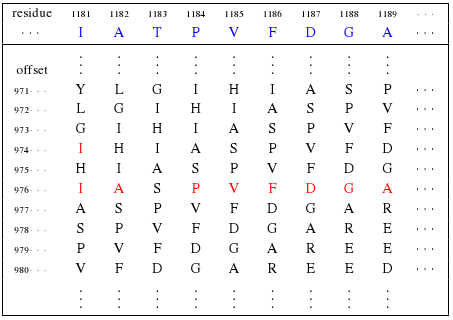
\includegraphics[]{offsets.png}}
% 	\caption{This is a subset of the binary 'bit matrix' constructed when comparing our two genes. The blue letters represent residues 1181-1189 of our sequence of interest. We are looking at a small section of the rows represented by offsets of 971-980. A red letter represents a match. As we can see there is an area of possible alignment in offset 976 as there are many more matches than we would believe to be expected.}
% 	\label{fig:00}
% \end{figure}
% \end{center}

\section{First filter: Global}

Now that we have this $(L_{S} + L_{T}-2w) \times (\min(L_{S},L_{T}))$ binary matrix $M$, we want to find what offsets result in abnormal quantities of matches. We want to find the rows in the matrix that have a higher than expected number of ones in them. To do this we take the sum of each row and compare it to the expectation of the number of matches based on amino acid frequency between that offset of the test sequence and the sequence of interest using a random model. If the sum of the ones is higher than some predetermined multiple of standard deviations away from the mean then it is marked as having a possible alignment. A default value of 3.5 assures that false positives should be extremely rare. We mark a row $i$ if,
\begin{equation}
    \sum_{j} M_{ij} > E\left(\sum_{j} A_{ij}\right) + \alpha \sqrt{E\left(\sum_{j} A_{ij}\right)}.
\end{equation}
where $E(X)$ is the expectation of $X$, $A_{i:}$ is a random vector constructed from sequences with the same amino acid composition, $\alpha$ is a parameter and is set to 3.5 by default and the square root represents the standard deviation (we assume a Poisson distribution). The value of 3.5 ensures a false positive rate of less than 0.1\% and we only look at one side distribution, offsets with higher than expected matches. The value of the mean and expectation is calculated analytically by combinatorially looking at all possible permutations of the test sequence. See figure 2.

We note that as the lengths of the sequences grow large the signal can become lost in the noise. Even a $k$-mer of length 1Kbp would be lost when comparing a 3Gbp sequence using this method. To account for this and also to make easier use of the Graphics Processing Unit (GPU) implementation of this algorithm, which enforces strict memory constraints, we break up the sequences into chunks of length 1000 before forming the matrix $M$. This not only ensures that the noise will not overwhelm the signal, but also allows for much faster, parallel implementations. Areas of similarity that extend over a separation are rejoined in the recompilation step. By only looking over a linear number of offsets in the length of the test sequences we achieve scaling of
$\mathcal O$($N$) where $N$ is the total length of the sequences
being compared. This is far less computationally complex than the alternative dynamic programming and HMM based methods.

[FIGURE 2 HERE]

% \begin{figure}[!tpb]%figure2
% \centerline{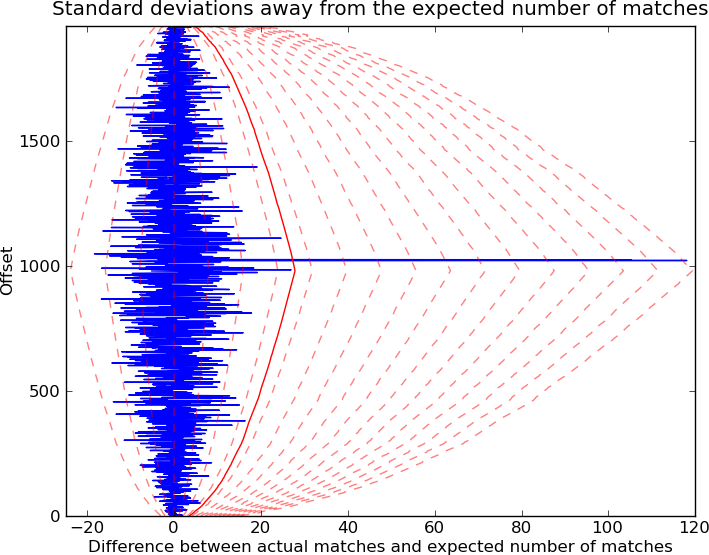
\includegraphics[]{globalFilterDuo.png}}
% 	\caption{Values of sums of rows of the bit matrix plotted against standard deviations from the mean. The right picture is a zoom in of the area where all 4 qualifying offsets lie.}
% 	\label{fig:01}
% \end{figure}

\section{Second filter: Local}

We now have the set of offsets that have a significant number of ones in them. The next goal is to quickly find where the areas of high density are in these vectors, if such areas exist, as these would be areas of high homology between the sequences. This is done by taking a running sum of each vector from its start, at each point we subtract off the expectation based on the amino acid frequency of the two sequences for each position. This has an effect of calculating how many ones have been found at or before that position above the number that would be expected. We know that this value must increase at some point in the vector because at the end there needs to be some extra number of ones equal to some number of standard deviations away from the mean, based on it passing the global step. Where this value peaks is where the club starts (is has a significant jump in the running sum over some window). When the value flattens out again that part of the sequence is no longer in the club. See Figure 3.

Two parameters are used here (combined with the one from the global filter they represent all three parameters of the model), the width of the block used for approximating the derivative and how many matches above the expectation are needed to trigger the start of the region. We can get the quick, bitwise location of the high density region in the vector, which corresponds to our in the club region. A useful side effect of this filter is that if there is no region of high density, if we have just accidentally found an outlier from the global filter that just happens to have a lot of sparse matches, then it will not trigger and we will not get a false positive from the result of the global step.

[FIGURE 3 HERE]

% \begin{figure}[!tpb]%figure3
% \centerline{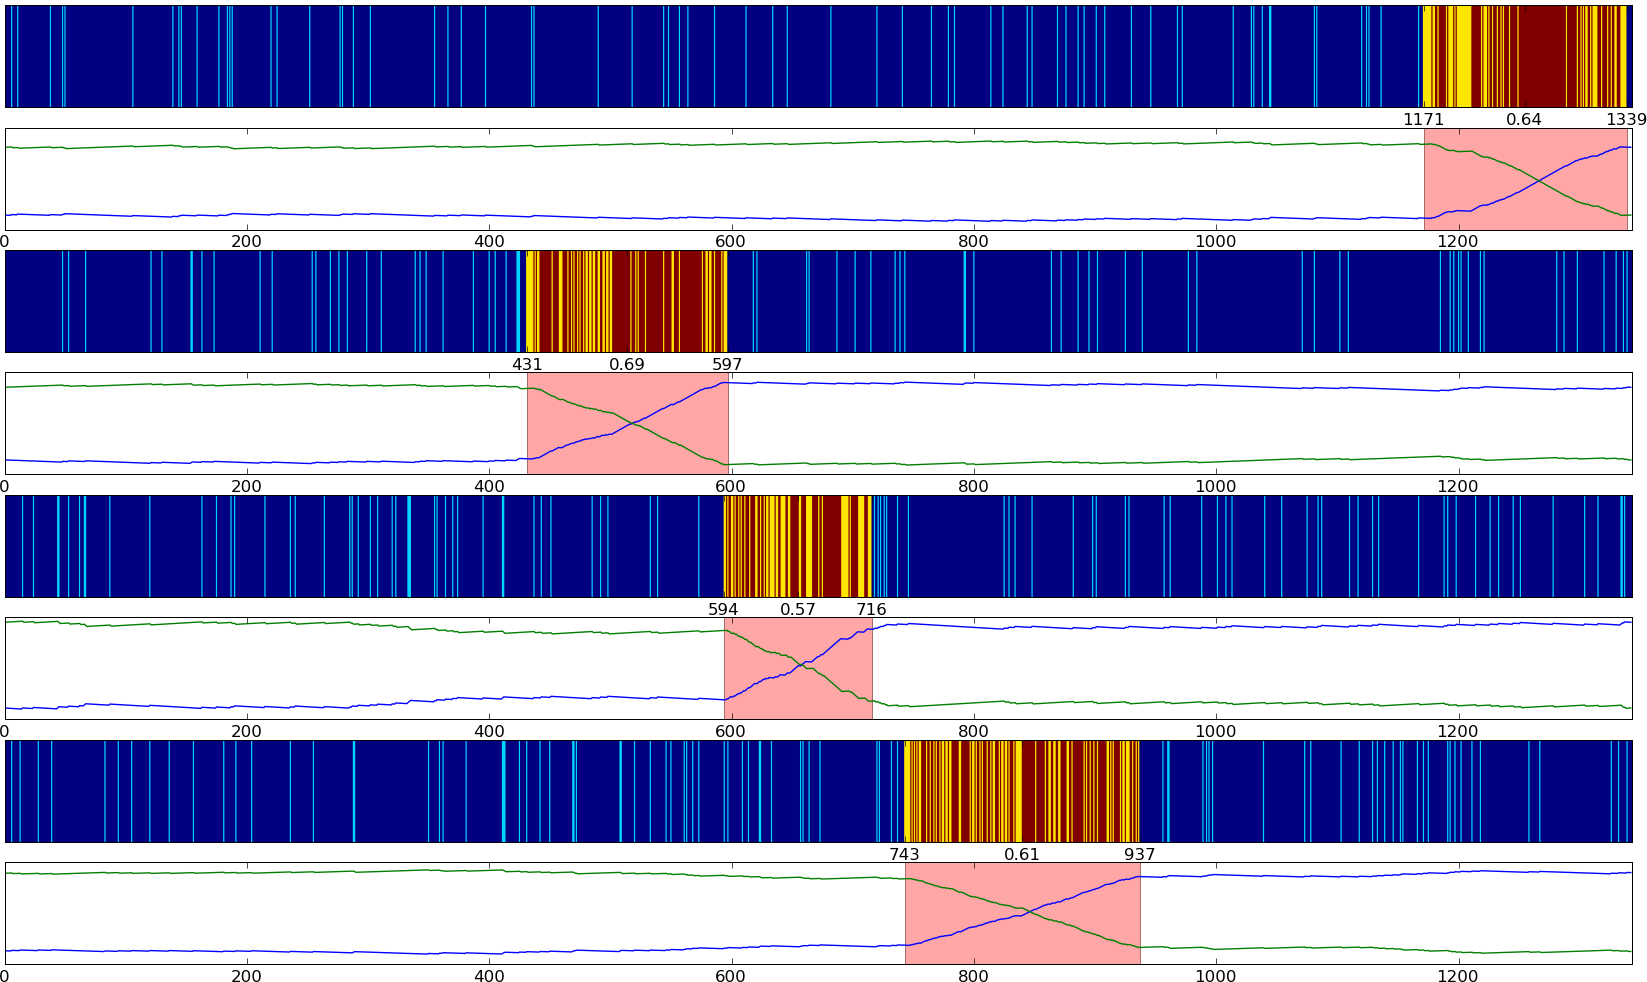
\includegraphics[]{localAlignmentsCDF.png}}
% 	\caption{The four vectors that passed the global filter test and their running sum calculation. When the approximate derivative of the running sum reaches a certain point the region is marked as having a possible alignment and shaded. For the vector blue means no match an not in that region, cyan is a match but not in the region (random match), yellow is the region of possible alignment and red are the positions in that region that have matches. The location of the region is marked along with the total density of matches within that region.}
% 	\label{fig:02}
% \end{figure}

\section{Recompilation}

Now we have the regions where we have reason to believe that there are local alignments between the two sequences, our in club areas. We can see where they lie on their respective sequences and how their densities compare with each other and the sequences as a whole. This can be important information because the shifting of conserved regions and possible transposition events can represent evolutionary distance between the sequences. If we consider the conserved regions to be fixed by natural selection then their relative drift away from each other should be related to when they originally diverged. We can see an example of this in Figure 4 where there is a difference in the sequence length between conserved areas of sequence.

[FIGURE 4 HERE]

% \begin{figure}[!tpb]%figure4
% \centerline{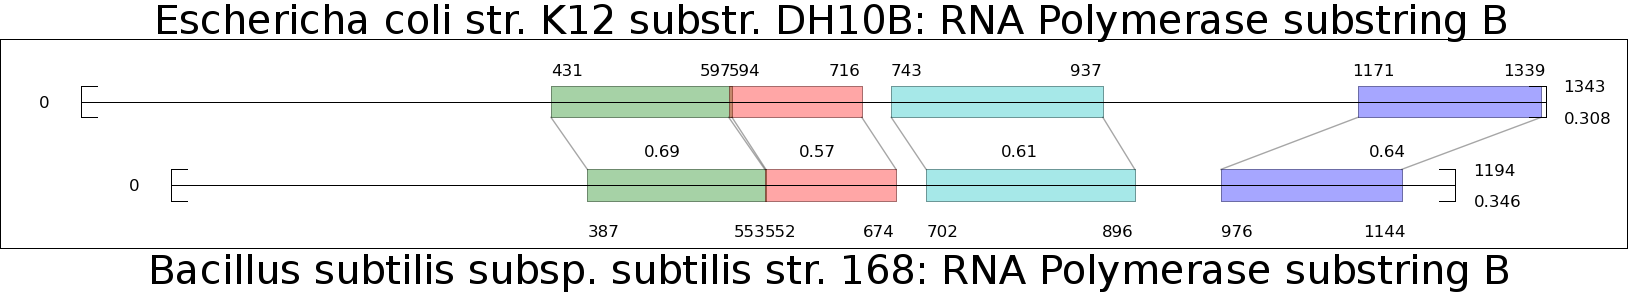
\includegraphics[]{localAlignmentsBreakout.png}}
% 	\caption{Above we see where each area of possible local alignment lies within the sequence of interest (top) and the test sequence (bottom) along with their respective positions and densities}
% 	\label{fig:03}
% \end{figure}

% chapter Velvetrope Methods (end)

\chapter{Velvetrope Results} % (fold)
\label{cha:Velvetrope Results}

\section{Multiple Sequence Alignment}

Multi-domain proteins have traditionally been cumbersome to Multiple Sequence Alignment (MSA) algorithms like MUSCLE \cite{MUSCLE} and DIALIGN-TX \cite{DIALIGN-TX} like the 31 multi-domain lectin proteins in Reference 8 of BAliBASE v3 \cite{Balibase}. The two domains for lectin are transposed for 4 of the organisms and are ordered ``correctly'' for the other 27 in the reference database (See figure 5). Because Velvetrope works independent of order it allows us to find transposed domains from within a protein such as this with relative ease and compute a probable, non-traditional MSA.

Comparing a sequence of interest against a large set of test sequences allows Velvetrope to find the areas within the sequence of interest that are homologous to multiple test sequences. By combining this information across many sequences (as in figure 6) we make a histogram of which residues were matches and in the club across many test sequences. We are able to discern areas of possible multiple alignment from within the sequence of interest in this fashion. By looking at the areas within the sequence of interest which are consistently identical to test sequences or in the club we can generate regular expressions of sequence that can be readily re-mapped onto the sequence of interest, representing a non-traditional multiple alignment.  This allows us to find a probable MSA and because Velvetrope only compares a single sequence of interest against a larger set we can use this to quickly append a new sequence to a multiple alignment multiple orders of magnitude faster than traditional methods which would have to recalculate the entire MSA for every appended sequence.

Traditional methods, like those in BAliBASE, have to be prompted with domain information to make sense of a multi-domain protein at all. Even with this information they only align the prompted domain and merely append the other domain(s) around the domain of interest. This results in a MSA that does not represent the true alignment between the proteins. Velvetrope is able to produce a shorter MSA with all domains represented without any prior information. In Figure 7 we look at two MSAs in which BAliBASE was prompted with the two lectin domains and it generates an non-intuitive alignment. While using just a single sequence of interest we are able to find both domains and re-map them onto that sequence and generate a much more compact and representative probable MSA very quickly.

[FIGURE 5,6,7 HERE]

% \begin{figure}[!tpb]%figure5
% \centerline{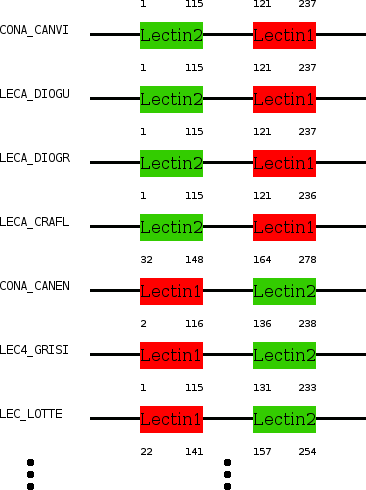
\includegraphics[]{BAliBASEsnap2v2.png}}
% 	\caption{The lectin sequences from \textit{Reference 8 - Circular Permutations} of BAliBASE3. The reference contains 31 two-domain lectin proteins from a myriad of organisms. In 4 of the sequences the Lectin2 domain comes before the Lectin1 domain, the opposite for the remaining 27. This presents a problem for most multiple alignment algorithms which will try to align one domain or the other.}
% 	\label{fig:04}
% \end{figure}
% 
% \begin{figure}[!tpb]%figure6
% \centerline{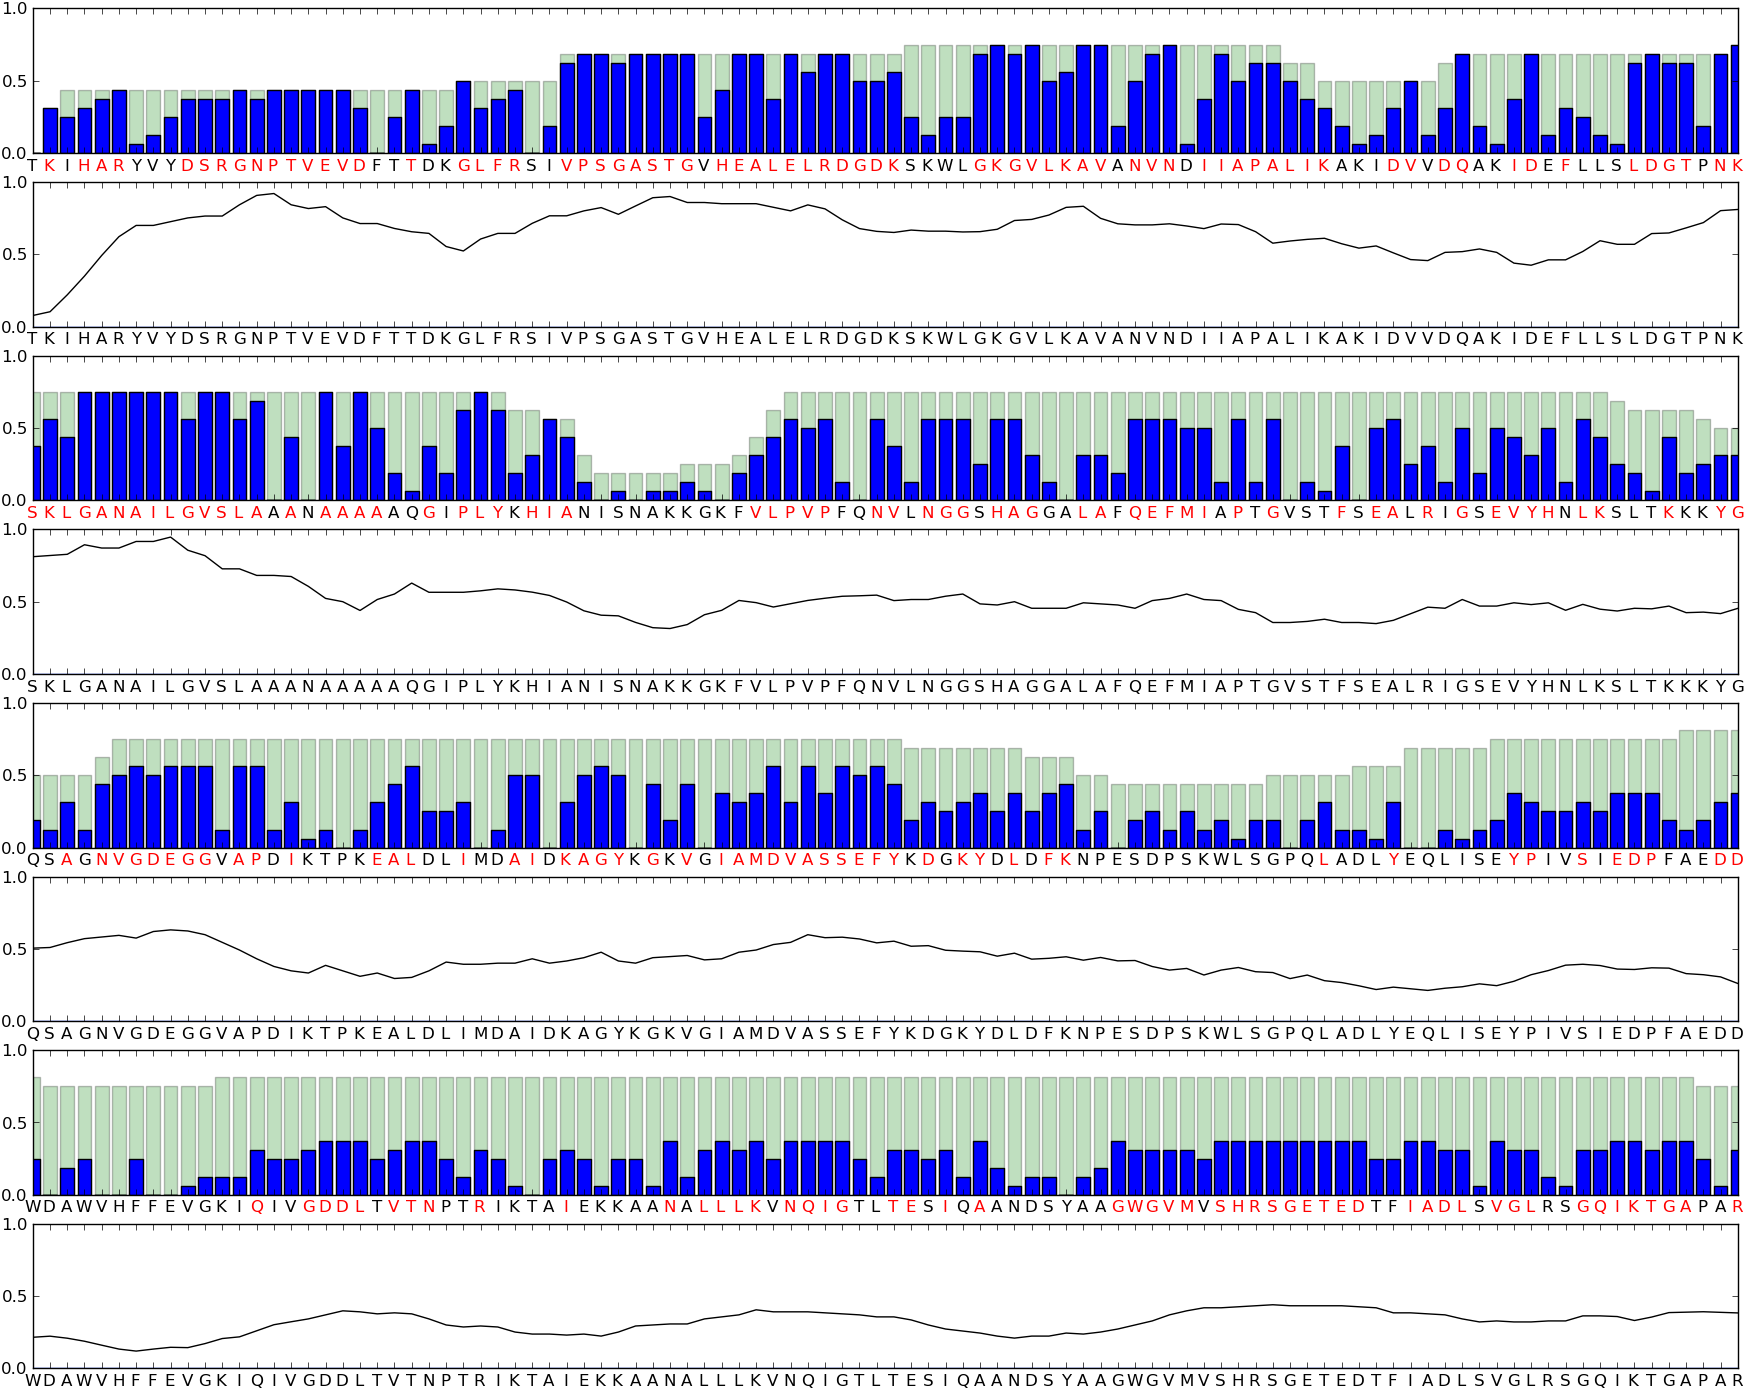
\includegraphics[]{COMBO1.png}}
% 	\caption{Add caption, talk about how you can get the regexp data from this and how we can see two domains...}
% 	\label{fig:05}
% \end{figure}
% 
% \begin{figure*}[!bpt]%figure6
% \centerline{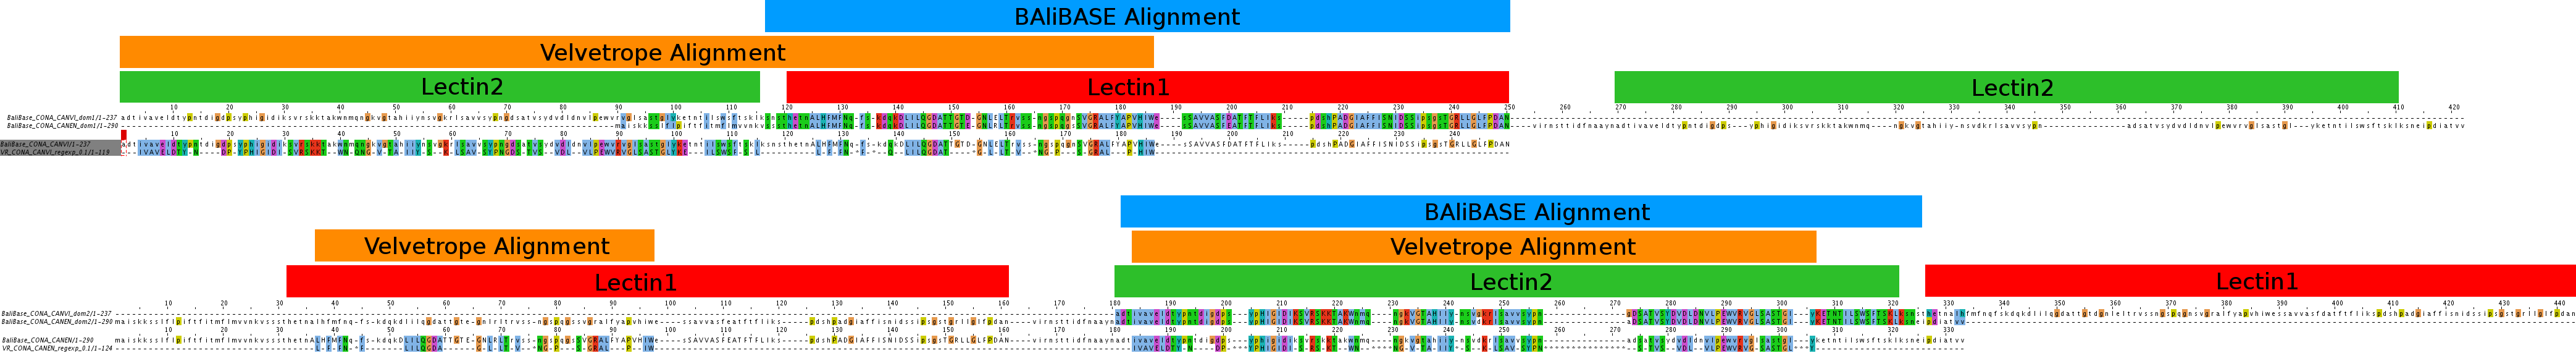
\includegraphics[]{Alignments.png}}
% 	\caption{Two sets of alignments of the two-domain lectin protein reference. Red corresponds to the Lectin1 domain. Green is the Lectin2 domain. Orange is the Velvetrope alignment. Blue is the BAliBASE alignment. BAliBASE resolves the two-domain problem by manually specifying which domain to align (Lectin1 in the first alignment, Lectin2 in the second). This causes the aligner to append whatever domain not specified to the beginning or end of the alignment. Velvetrope is order independent which allows it to pick out areas of homology regardless of position in the sequence without any expert tuning. Lectin1 suffers from low homologous identity in the latter part of its domain and is therefore not picked up by Velvetrope, but is aligned by the non-homology components of BAliBASE.}
% 	\label{fig:05}
% \end{figure*}


\section*{Local alignment comparison}

While Velvetrope does not perform a local alignment in the traditional sense it is able to find areas of high local homology between sequences, regardless of order or k-mer density, that are highly probable areas of local alignment. Velvetrope compares well at a visual level to standard algorithms like BLAST \cite{BLAST} and HMMer \cite{Eddy98} and the C/CUDA implementation executes at the same order of magnitude or faster than these methods. Velvetrope is very susceptible to high indel rates within a conserved region (shifts the offsets) but has been shown to equal or outperform these other methods in areas of low indel rate especially when there are only short $k$-mers within the homologous region between the two sequences.

% chapter Velvetrope Results (end)

\chapter{Velvetrope Implementation} % (fold)
\label{cha:Velvetrope Implementation}

Velvetrope is able to find areas of sequence homology quickly and efficiently across multiple sequences. It finds these areas of high shared identity density in a way that allows it to locate areas otherwise missed by $k$-mer based or position dependent methods. It is able to correctly find probable alignments in multi-domain proteins and pairwise local areas of similarity between distant homologies. Its low order of computational complexity, $\mathcal O$($N$) where $N$ is the total length of the sequences
being compared, allows for it to scale with the data intensive challenges that fields like metagenomics and cancer genomics present.

We also present a freely available, open source implementation (both serial and parallel; in Python, C and CUDA) with easy to navigate HTML output similar to MEME \cite{MEME}. The API and documentation make it easily extendable and able to adapt to the future computationally intensive problems it is designed to address.

\section{Availability and requirements}
 \begin{itemize}
  \item \textbf{Project name:} Velvetrope
  \item \textbf{Project home page:} velvetrope.sourceforge.net
  \item \textbf{Operating systems:} Linux 32/64-bit, Mac OSX, Windows (Cygwin)
  \item \textbf{Programming languages:} Python, C, CUDA, HTML/CSS
  \item \textbf{Other requirements:} Some python packages, see documentation
  \item \textbf{License:} GPL v2.01
 \end{itemize}

% chapter Velvetrope Implementation (end)

% part Velvetrope (end)

\appendix
\chapter{Chapter 1 of appendix}
Appendix chapter 1 text goes here

\bibliography{ScottClark_thesis}

\end{document}
